\section{The modular tessellation of the upper halfplane}

Since $\FunSet$ is a fundamental set for the action of $\PSL{\Z}$ on $\EU$, its images under all modular transformations cover the extended upper halfplane $\EU$ -- compare also Remark~\ref{rem_FunSetUniqueElement}. Thus for a point $z \in \EU$ there exists a transformation $A \in \PSL{\Z}$ such that $z \in A\FunSet$. We can effectively determine such a transformation by adopting the algorithm of Theorem~\ref{thm_SL2FunDomAlg}:

\begin{theorem}[The fundamental set algorithm]
Let $z \in \EU$ be a point of the extended upper halfplane and let the fundamental set $\FunSet$ be defined as in (\ref{eqn_PSL2FunSet}). A transformation $A$ satisfying $z \in A \FunSet$ can be found by performing the following steps:
\begin{enumerate}
\item Set $j := -1$ and $B_0 := 1$.
\item \label{itm_PSL2FunSetAlgLoop}
Increment $j$ by one and set $z_j := B_j z$. If $z_j \in \FunSet$, then goto step \ref{itm_PSL2FunSetAlgDone}.
\item \label{itm_PSL2FunSetAlgEjDef}
Set $e_j := \floor{\Re{z_j} + \reci{2}}$. 
\item \label{itm_PSL2FunSetAlgNext}
If $z_j - e_j \in \FunSet$, set $B_{j+1} := U^{-e_j}B_j$ -- else set $B_{j+1} := TU^{-e_j}B_j$.
\item Continue with step \ref{itm_PSL2FunSetAlgLoop}.
\item \label{itm_PSL2FunSetAlgDone} 
The desired matrix $A$ is given by $A = \inv{B_j}$.
\end{enumerate}
\end{theorem}
\begin{proof}
Note that the above is essentially a reformulation of the algorithm of Theorem~\ref{thm_SL2FunDomAlg} with the following modifications:
\begin{enumerate}[\quad (a)]
\item The algorithm is reformulated for the inhomogeneous case. The numbers $z_j$ from above and the vectors $x_j$ from the proof of Theorem~\ref{thm_SL2FunDomAlg} correspond by $z_j = \pi(x_j)$.
\item \label{itm_PSL2FunDomAlgModNint}
Instead of using the $\nint{}$ function, we use the above definition  for determining the coefficients $e_j$ -- see step \ref{itm_PSL2FunSetAlgEjDef}. This is to ensure that $z_j - e_j \in [-\reci{2}, \reci{2})$ -- otherwise we would have problems with the termination of the algorithm for the case when some $z_j$ lies on the boundary arc $b$ (as defined in Theorem~\ref{thm_PSL2FunSet}).
\item Theorem~\ref{thm_SL2FunDomAlg} yields a final vector $x_n$ such that $w := \pi(x_n) \in \topcl{\mathcal{R}}$, where $\mathcal{R}$ is defined as in (\ref{eqn_PSL2MinRegion}). In order to obtain a point in $\FunSet \subseteq \topcl{\mathcal{R}}$, we need to apply to $w$ possibly $T$ and -- if this point lies on the boundary arc $b$ -- possibly $U^{-1}$. We take this into account by explicitly checking whether the application of $T$ in the last iteration of the algorithm is necessary or not (see step \ref{itm_PSL2FunSetAlgNext}) and by the modification discussed in (\ref{itm_PSL2FunDomAlgModNint}).\qedhere
\end{enumerate}
\end{proof}

\begin{figure}
\centering
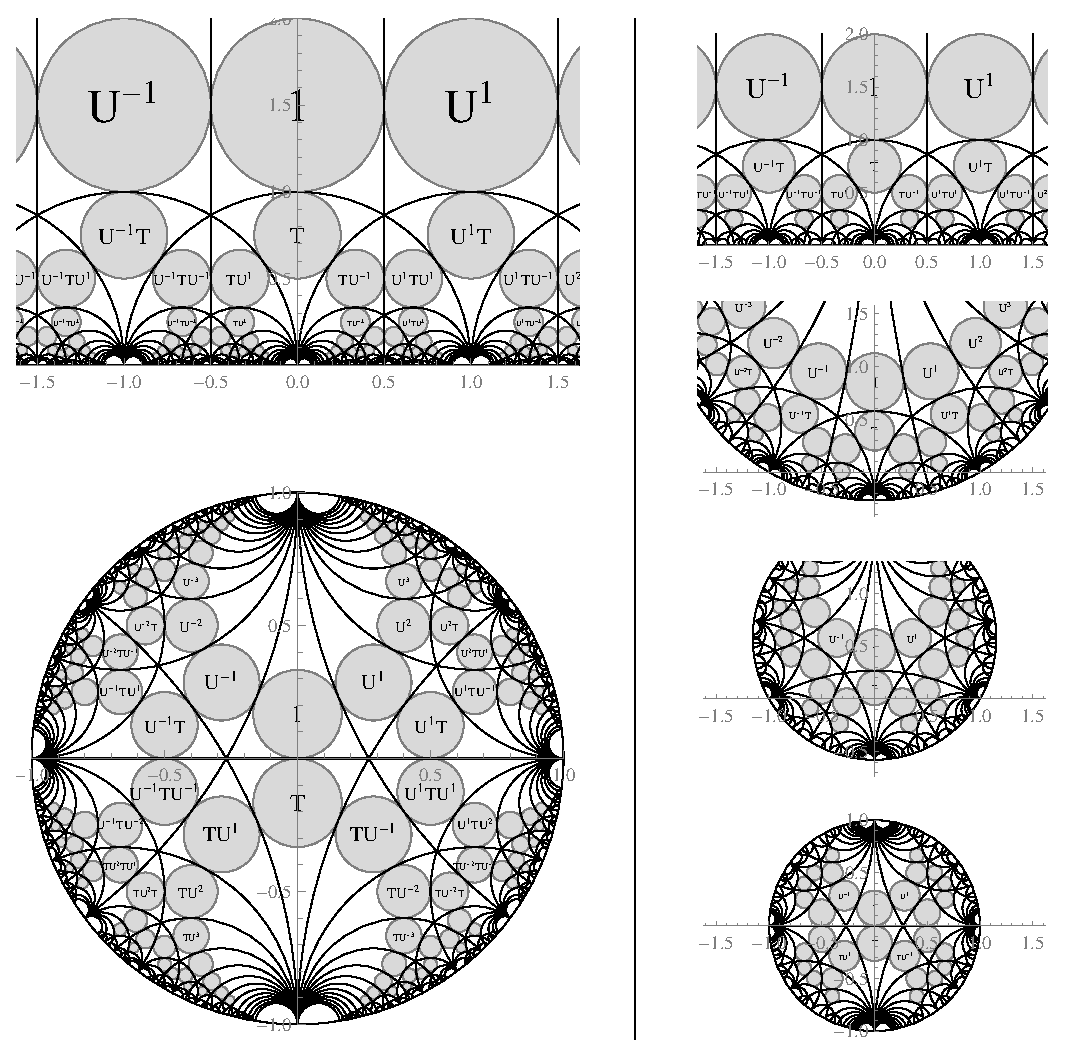
\includegraphics[width=\textwidth]{figures/modular-tiling-1}
\caption{The modular tessellation. The images of the fundamental region $\FunDom$ and its indisk $\Indisk$ under all modular transformations (top left) are mapped to the unit circle by the modified Cayley transform $\ModCayley$ (bottom left). A continuous transition between these images is induced by a quarter-turn of the Riemann sphere and can be seen on the right.}
\label{fig_ModularTiling}
\end{figure}
\index{Tessellation}
\index{Modular!tessellation}
In Figure~\ref{fig_ModularTiling} on the top-left, we see the images of the fundamental region $\FunDom$ and its indisk $\Indisk$ under the transformations of the modular group. Each of these images $A \FunDom$ \resp $A \Indisk$ is labeled by the $T$-$U$ word representation of the corresponding transformation $A \in \PSL{\Z}$. We call the covering of $\EU$ by images of $\FunSet$ the \emph{modular tessellation} of the upper halfplane.

For visualization purposes, the upper halfplane has the obvious disadvantage that we can never see the whole picture. We have seen in Example~\ref{ex_ModCayleyTransform} that the modified cayley transform $\ModCayley$ maps the upper halfplane to the unit disk. We can therefore use $\ModCayley$ to translate the modular tessellation to the unit disk. This means instead of looking at the regions $A \FunDom$ \resp $A \Indisk$ for all $A \in \SL{\Z}$, we can alternatively depict the regions $\ModCayley A \FunDom$ and the corresponding indisks $\ModCayley A \Indisk$ which is done in the bottom-left picture of Figure~\ref{fig_ModularTiling}. 

For a better understanding of this transformed representation of the modular tessellation, let us identify the drawing area with $\R^2$ rather than with $\C$. Now we note that the point $(0,1)$ corresponds to the point $\infty \in \EU$, the points $(\pm 1, 0)$ relate to $\pm 1 \in \EU$ respectively and the point $(0,-1)$ refers to $0 \in \EU$. The center $(0,0)$ represents the imaginary unit $\ii \in \EU$. In other words, as can be seen in the right column of Figure~\ref{fig_ModularTiling}, $\ModCayley$ bends the real axis to a circle\footnote{In fact, the real axis plus the point $\infty$ can be considered as generalized circle already.}, gluing together its ends at the point $\infty$ and enclosing the upper halfplane in its interior. As we have seen in Example~\ref{ex_ModCayleyTransform}, this continuous transition between the tessellation on the upper halfplane and its image under $\ModCayley$ can be explained by a quarter-turn of the Riemann sphere -- compare also Figure~\ref{fig_StereoProjModCayley}.

\begin{remark}
In a more formal context, the bottom-left picture of Figure~\ref{fig_ModularTiling} can also be interpreted in two alternative ways: Firstly, we could consider a different action of $\PSL{\Z}$ on $\EC$, which we may denote as $A \ast z$ for $A \in \PSL{\Z}$ and $z \in \EC$. For its definition we make use of the natural action of the M�bius transformation $\ModCayley A \inv{\ModCayley}$:
\begin{equation*}
A \ast z := (\ModCayley A \inv{\ModCayley}) z.
\end{equation*}
Secondly, we could consider $\EC$ under the natural action of a group $G$ of M�bius transformations which is conjugate to $\PSL{\Z}$ and whose transformations are represented by certain matrices over the ring of Gaussian integers $\Z[\ii]$ with determinant 1:
\begin{equation*}
G := \ModCayley \PSL{\Z} \inv{\ModCayley} = \setdefsz{\bigg}{A \in \PSL{\Z[\ii]}}{A = \mat{\alpha}{\beta}{\conj{\beta}}{\conj{\alpha}}_\sim}.
\end{equation*}
Clearly both, the action $\ast$ of $\PSL{\Z}$ as well as the natural action of $G$, leave the unit disk $\ModCayley \mathcal{H}$ invariant. Consequently $\ModCayley \FunDom$ is a fundamental region for both (equivalent) actions on the unit disk. Now the bottom-left picture of Figure~\ref{fig_ModularTiling} can be interpreted as the tessellation induced by either of these two group actions.
\end{remark}
